%%%%%%%%%%%%
\section{RFSoC signal transmitter}
%%%%%%%%%%%%%%%%%%%%%%%%%%%%%%%%%%%%%%%%%%%
\begin{frame}{RFSoC signal transmitter}{}
	\begin{columns}
		\begin{column}{0.4\textwidth}
			\begin{block}{ZCU208}
			\end{block}
		\end{column}
		\begin{column}{0.6\textwidth}
			\begin{center}
				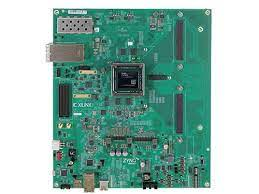
\includegraphics[scale=0.65]{graphics/zcu208.jpeg}
			\end{center}
		\end{column}
	\end{columns}
\end{frame}
%%%%%%%%%%%%%%%%%%%%%%%%%%%%%%%%%%%%%%%%%%%
\begin{frame}{RFSoC signal transmitter}{tx-subsystem}
	\begin{figure}
		\centering
		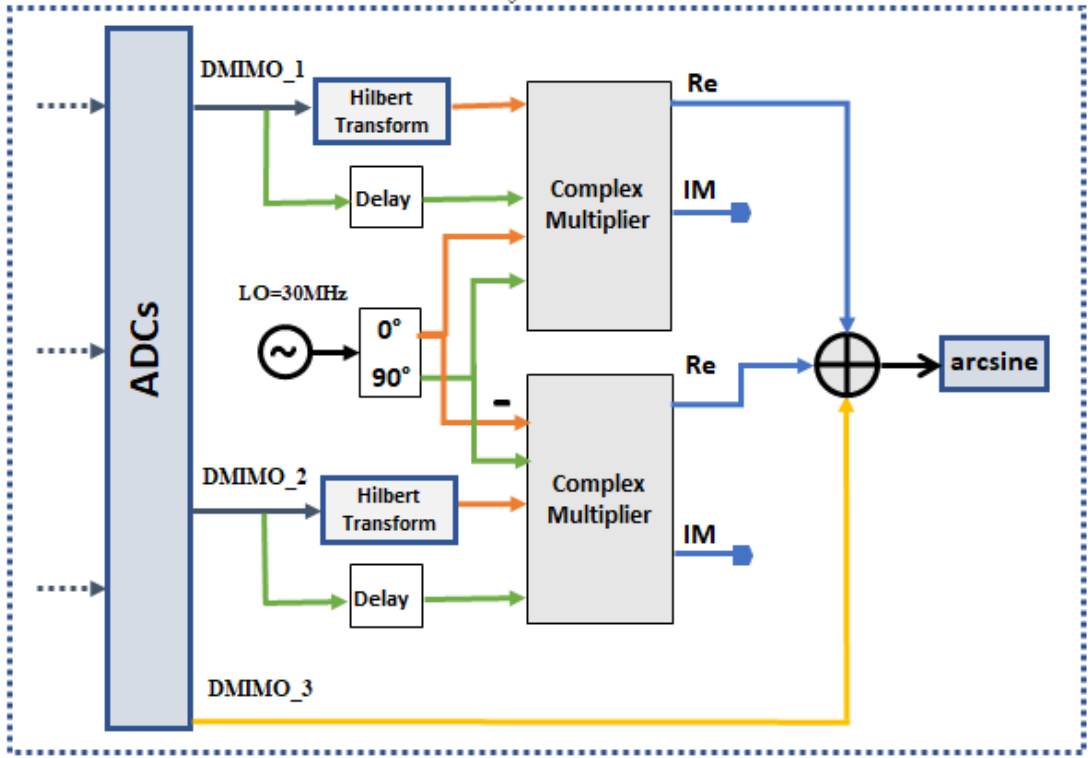
\includegraphics[scale=1]{graphics/tx_ss.png}
		\caption{transmitter subsystem}
	\end{figure}
\end{frame}
%%%%%%%%%%%%%%%%%%%%%%%%%%%%%%%%%%%%%%%%%%%
\begin{frame}{RFSoC signal transmitter}{rx-subsystem}
	\begin{figure}
		\centering
		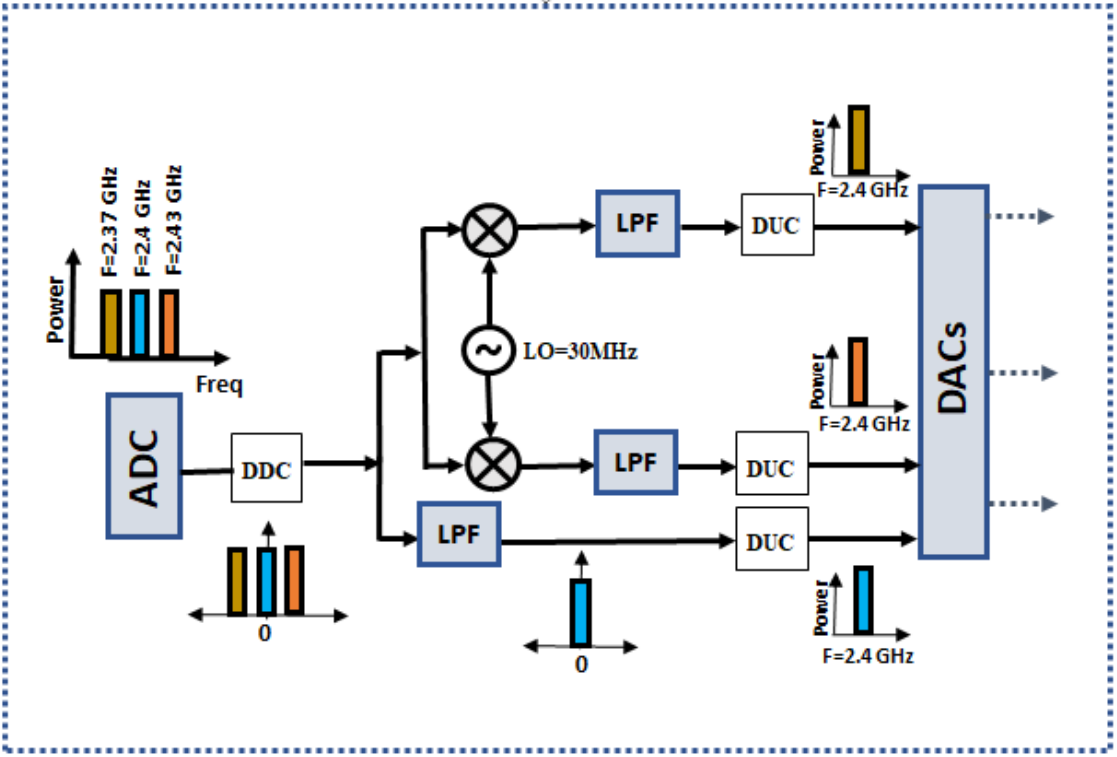
\includegraphics[scale=1]{graphics/rx_ss.png}
		\caption{Receiver subsystem}
	\end{figure}
\end{frame}
%%%%%%%%%%%%
\section{Real-time Spectrum Analyzer}
%%%%%%%%%%%%%%%%%%%%%%%%%%%%%%%%%%%%%%%%%%% 
\begin{frame}{Real-time Spectrum Analyzer}{}
	\begin{block}{Spectrum analyzer type:}
		\begin{itemize}
			\item Swept-tuned spectrum analyzer
			\item Vector signal analyzers
			\item Real-time spectrum analyzers (RTSA)
		\end{itemize}
	\end{block}
	\pause
	\begin{block}{}
		Real-time spectrum analysis allows a spectrum analyzer to conduct continuous,
		gapless capture and analysis of elusive and transient signals, while conventional
		spectrum analyzers and vector signal analyzers do not have this capability due to their design.
	\end{block}
\end{frame}
%%%%%%%%%%%%%%%%%%%%%%%%%%%%%%%%%%%%%%%%%%%
\begin{frame}{Real-time Spectrum Analyzer}{Swept-tuned spectrum analyzer}
	\begin{figure}
		\centering
		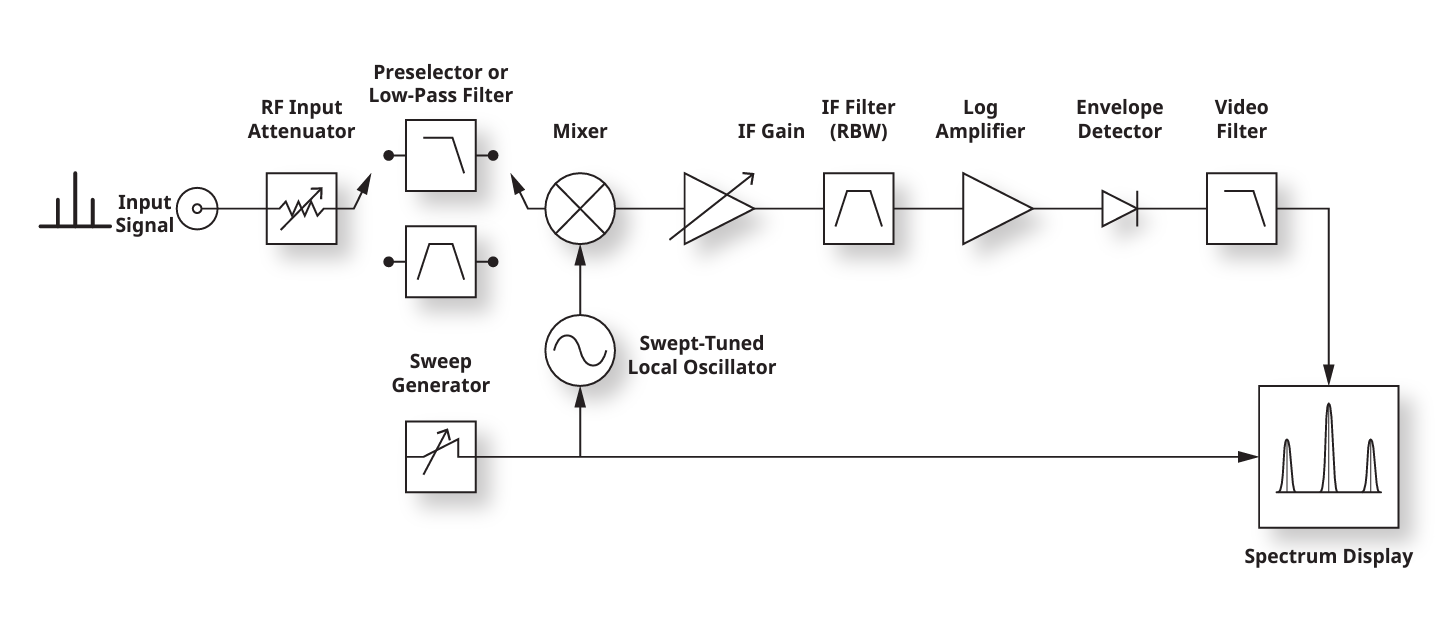
\includegraphics[scale=0.9]{graphics/rtsa_fig1_1.png}
		\caption{Diagram of a classic swept-tuned spectrum analyzer}
	\end{figure}
\end{frame}
%%%%%%%%%%%%%%%%%%%%%%%%%%%%%%%%%%%%%%%%%%%
\begin{frame}{Real-time Spectrum Analyzer}{Swept-tuned spectrum analyzer}
	\begin{figure}
		\centering
		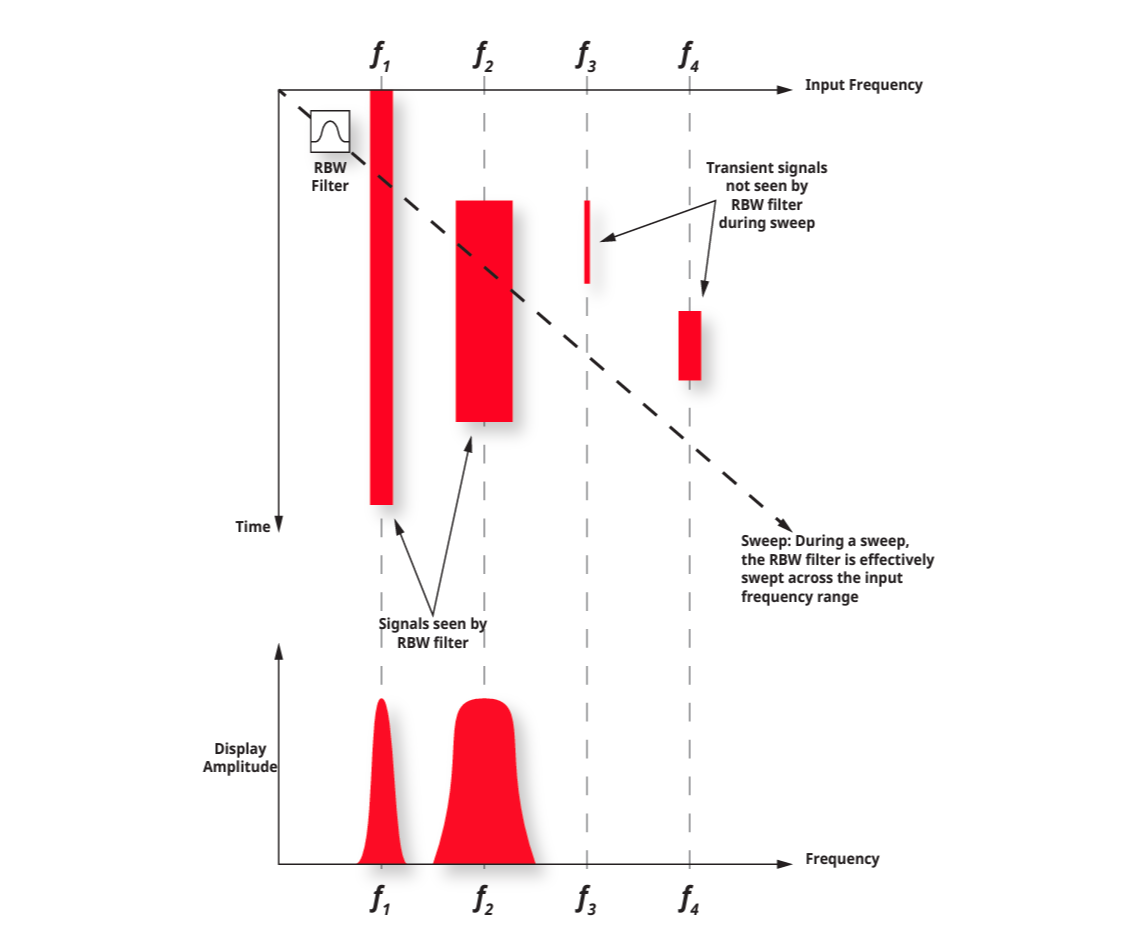
\includegraphics[scale=0.65]{graphics/rtsa_fig1_2.png}
		\caption{Swept-tuned spectrum analyzer response to transient signals during a sweep}
	\end{figure}
\end{frame}
%%%%%%%%%%%%%%%%%%%%%%%%%%%%%%%%%%%%%%%%%%%
\begin{frame}{Real-time Spectrum Analyzer}{Vector signal analyzer}
	\begin{figure}
		\centering
		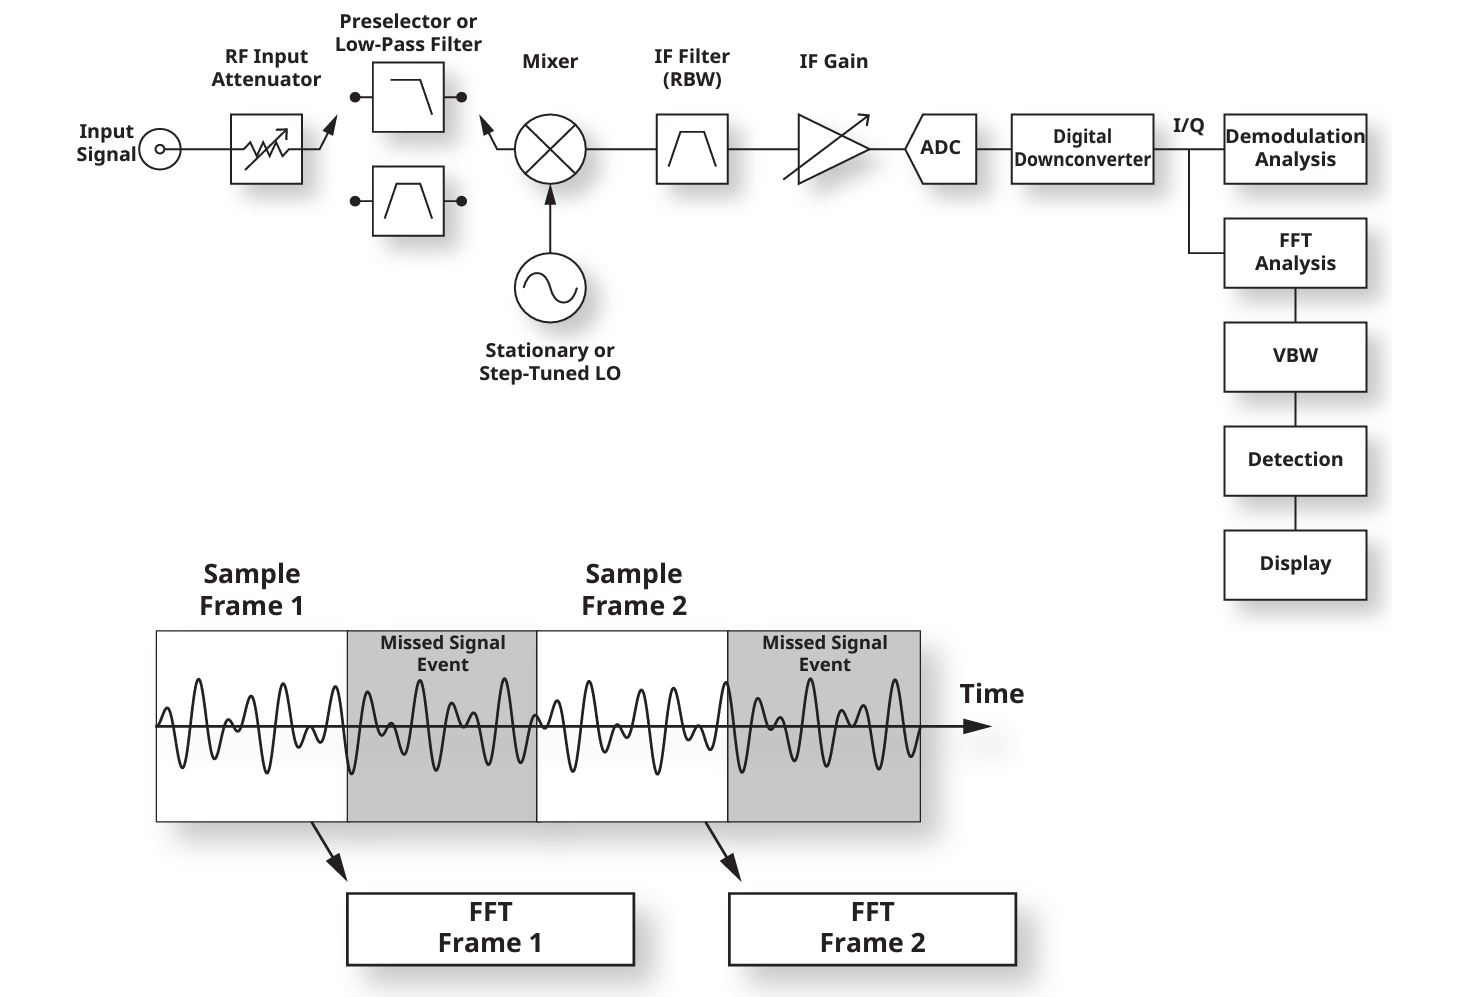
\includegraphics[scale=0.7]{graphics/rtsa_fig2.png}
		\caption{Block diagram of simplified vector signal analyzer and signal processing flow}
	\end{figure}
\end{frame}
%%%%%%%%%%%%%%%%%%%%%%%%%%%%%%%%%%%%%%%%%%%
\begin{frame}{Real-time Spectrum Analyzer}{RTSA}
	\begin{figure}
		\centering
		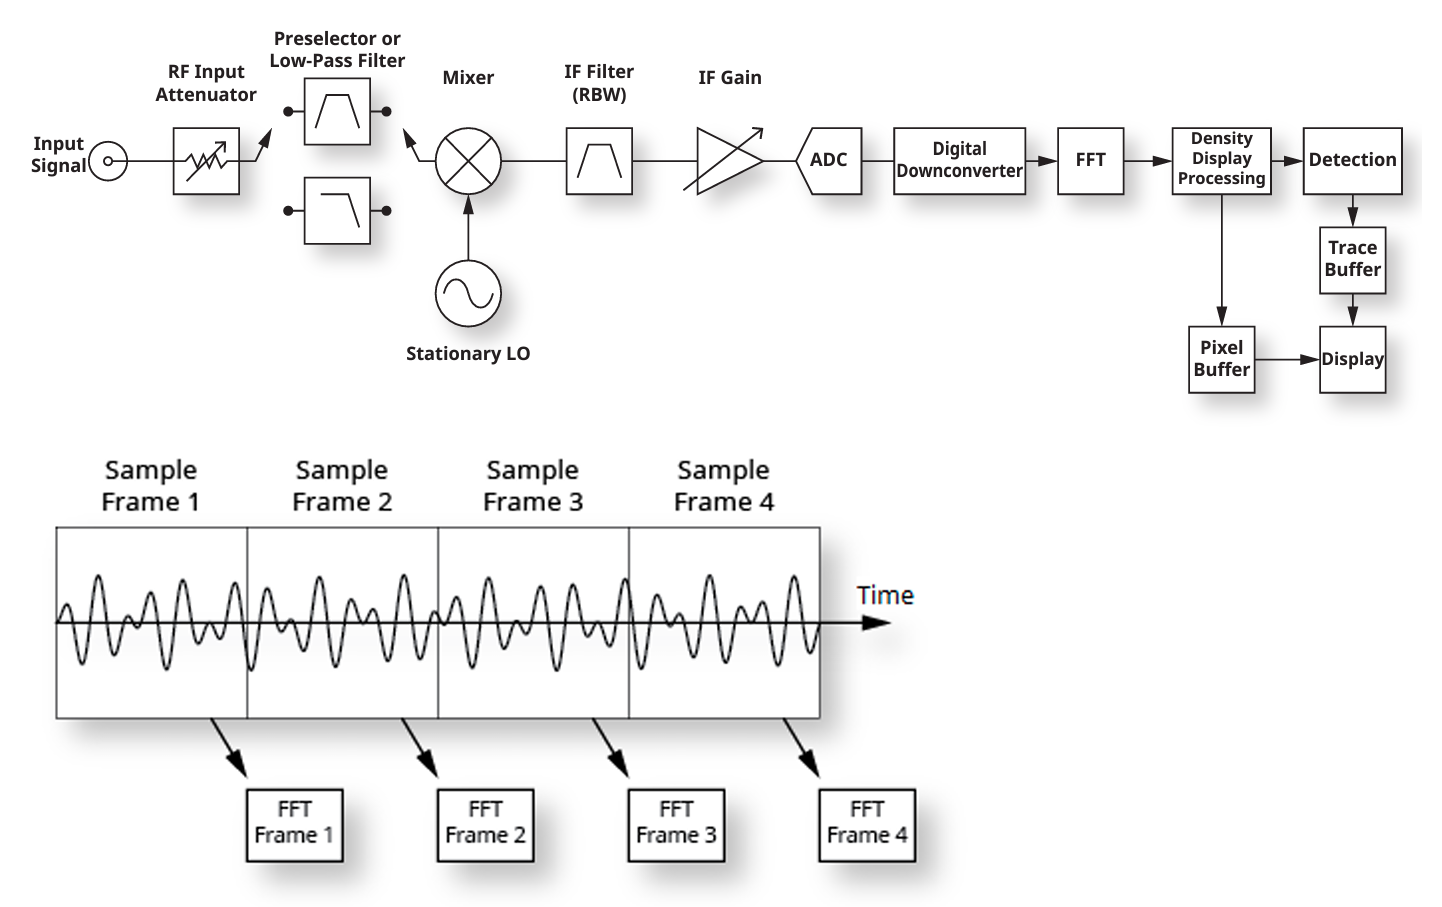
\includegraphics[scale=0.7]{graphics/rtsa_fig3.png}
		\caption{Real-time spectrum analyzer block diagram and signal processing flow}
	\end{figure}
\end{frame}
%%%%%%%%%%%%%%%%%%%%%%%%%%%%%%%%%%%%%%%%%%%
\begin{frame}{Real-time Spectrum Analyzer}{3D-Histogram}
	\begin{figure}
		\centering
		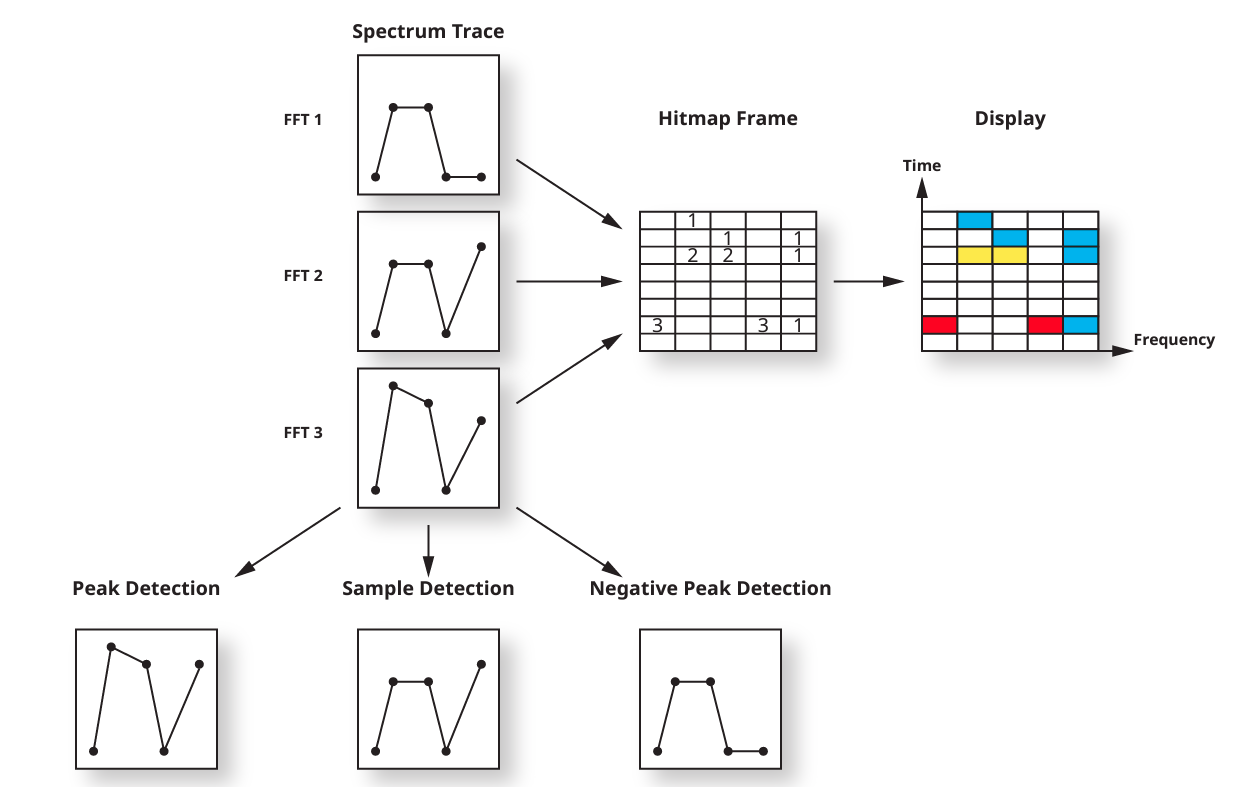
\includegraphics[scale=0.85]{graphics/rtsa_fig4.png}
		\caption{Shows how the spectrum traces are constructed from the detected
			amplitude of all three FFTs acquired during the acquisition time interval}
	\end{figure}
\end{frame}
%%%%%%%%%%%%%%%%%%%%%%%%%%%%%%%%%%%%%%%%%%%
\begin{frame}{Real-time Spectrum Analyzer}{Implementation}

\end{frame}






